\documentclass[journal]{IEEEtran}
\usepackage[a5paper,margin=10mm]{geometry}
\setlength{\headheight}{1cm}
\setlength{\headsep}{0mm}

% Use the same GVV layout and mathematical notation as the Class 10 project.
\usepackage{gvv-book}
\let\savedvec\vec
\usepackage{gvv}
\let\vec\savedvec
\usepackage[center]{caption}
\raggedbottom
\hypersetup{colorlinks=true,urlcolor=black,linkcolor=black,citecolor=black,hypertexnames=false,pdftitle={CBSE Class 12 Mathematics 2015}}
\makeindex

\renewcommand{\myvec}[1]{\ensuremath{\begin{bmatrix}#1\end{bmatrix}}}
\renewcommand{\mydet}[1]{\ensuremath{\begin{vmatrix}#1\end{vmatrix}}}
\renewcommand{\solution}{\par\smallskip\noindent\textbf{Solution.}\;}
\newcounter{qcurrent}

\begin{document}
\bibliographystyle{IEEEtran}
\onecolumn
\title{\begin{center}{\LARGE\bfseries Math for EE}\\\rule{0.4\columnwidth}{0.4pt}\end{center}}
\author{\vspace{11cm}\begin{center}{\fontsize{26}{31}\selectfont\bfseries CBSE Class 12 2015}\end{center}}
\maketitle
\thispagestyle{empty}
\newpage
\tableofcontents
\newpage

\section{Formulae}
\paragraph*{Vectors and three-dimensional geometry}
For vectors $\vec a,\vec b\in\mathbb R^3$,
\begin{align}\intertext{\textbf{1.1.5}}
\vec a\cdot\vec b&=a_1b_1+a_2b_2+a_3b_3,\quad \vec a\perp\vec b\iff \vec a\cdot\vec b=0. \tag{1.1.5.1}\\
\intertext{\textbf{1.1.1}}
\vec a\times\vec b&=\begin{pmatrix}a_2b_3-a_3b_2\\a_3b_1-a_1b_3\\a_1b_2-a_2b_1\end{pmatrix}. \tag{1.1.1.1}\\
\text{unit vector along }\vec v&=\frac{\vec v}{\norm{\vec v}},\qquad \norm{c\vec v}=|c|\norm{\vec v}. \tag{1.1.1.2}
\end{align}
The vector product is normal to both vectors in the product. Distances and line/plane relations are
The cross product is perpendicular to both input vectors:
\noindent\textbf{1.1.5}\quad
\begin{equation}
\vec a\times\vec b\perp\vec a,\qquad \vec a\times\vec b\perp\vec b.\tag{1.1.5.2}\label{eq:cross-perpendicular}
\end{equation}
\begin{align}\intertext{\textbf{1.1.6}}
d(\text{parallel lines})&=\frac{\norm{(\vec b-\vec a)\times\vec v}}{\norm{\vec v}}. \tag{1.1.6.1}\\
\intertext{\textbf{1.1.2}}
d(\text{skew lines})&=\frac{|(\vec b-\vec a)\cdot(\vec v_1\times\vec v_2)|}{\norm{\vec v_1\times\vec v_2}}. \tag{1.1.2.2}\\
\intertext{\textbf{1.1.10}}
\text{line parallel to plane}&\iff \vec d\cdot\vec n=0. \tag{1.1.10.1}\\
\text{plane through }\vec r_0\text{ with normal }\vec n:\quad \vec n\cdot(\vec r-\vec r_0)&=0. \tag{1.1.10.2}\\
\intertext{\textbf{1.1.15}}
\text{line with point }\vec A\text{ and direction }\vec d:\quad \vec r&=\vec A+t\vec d. \tag{1.1.15.1}
\end{align}

\paragraph*{Matrices and determinants}
\begin{align}\intertext{\textbf{1.1.28}}
\det(AB)&=\det(A)\det(B),\qquad \det(A^n)=(\det A)^n. \tag{1.1.28.1}\\
\intertext{\textbf{1.1.30}}
A^{-1}&=\frac{\operatorname{adj}(A)}{\det A},\qquad \det A\ne0. \tag{1.1.30.1}\\
A\vec x=\vec b&\quad\Longrightarrow\quad \vec x=A^{-1}\vec b\quad(A\text{ invertible}). \tag{1.1.30.2}\\
\intertext{\textbf{1.1.37}}
[A\mid \vec b]&\xrightarrow{\text{elementary row operations}}[I\mid\vec x]\quad\text{(Gaussian elimination)}. \tag{1.1.37.1}
\end{align}
The identity used to factor the determinant in Q36 is
\noindent\textbf{1.1.36}\quad
\[
a^2+b^2+c^2-ab-bc-ca=\frac12\bigl((a-b)^2+(b-c)^2+(c-a)^2\bigr).\tag{1.1.36.1}
\]

\paragraph*{Differentiation and differential equations}
For $y' + P(x)y=Q(x)$, the integrating factor is
\noindent\textbf{1.1.24}\quad
\begin{equation}
\mu(x)=e^{\int P(x)\,dx}.\tag{1.1.24.1}\label{eq:if-24}
\end{equation}
The logarithmic derivative is
\noindent\textbf{1.1.40}\quad
\begin{equation}
\frac{d}{dx}\log|u(x)|=\frac{u'(x)}{u(x)},\qquad u(x)\ne0.\tag{1.1.40.1}\label{eq:log-derivative-40}
\end{equation}
The same identity gives
\noindent\textbf{1.1.42}\quad
\begin{equation}
\frac{d}{dx}\log|u(x)|=\frac{u'(x)}{u(x)},\qquad u(x)\ne0.\tag{1.1.42.1}\label{eq:log-derivative-42}
\end{equation}
\begin{align}\intertext{\textbf{1.1.25}}
\frac{dy}{dx}&=\frac{dy/dt}{dx/dt},\qquad \frac{d^2y}{dx^2}=\frac{d}{dt}(dy/dx)\bigg/\frac{dx}{dt}. \tag{1.1.25.2}\\
\intertext{\textbf{1.1.20}}
y'+P(x)y&=Q(x),\quad \mu(x)=e^{\int P(x)\,dx},\quad \frac{d}{dx}(\mu y)=\mu Q. \tag{1.1.20.1}\\
\intertext{\textbf{1.1.22}}
y=vx&\quad\Longrightarrow\quad y'=v+xv'\quad\text{(homogeneous first-order ODE)}. \tag{1.1.22.1}\\
\intertext{\textbf{1.1.21}}
(1+(y')^2)^3&=r^2(y'')^2\quad\text{for a circle family of fixed radius }r. \tag{1.1.21.1}\\
\intertext{\textbf{1.1.25}}
\frac{d}{dx}\log|u(x)|&=\frac{u'(x)}{u(x)},\qquad u(x)\ne0. \tag{1.1.25.1}
\end{align}

\paragraph*{Integration and area}
A useful definite-integral antiderivative is
\noindent\textbf{1.1.39}\quad
\begin{equation}
\int\frac{du}{a^2-u^2}=\frac1{2a}\log\left|\frac{a+u}{a-u}\right|+C.\tag{1.1.39.1}\label{eq:int-rational-39}
\end{equation}
After polynomial division, partial fractions can be written as
\noindent\textbf{1.1.43}\quad
\begin{equation}
\frac{P(x)}{(x-a)(x^2+b^2)}=Q(x)+\frac{A}{x-a}+\frac{Bx+C}{x^2+b^2}.\tag{1.1.43.1}\label{eq:partial-fractions-43}
\end{equation}
The trigonometric integrand in Question 44 can be split using
\noindent\textbf{1.1.44}\quad
\begin{equation}
\frac{5\sin x+3\cos x}{\sin x+\cos x}=4+\frac{\sin x-\cos x}{\sin x+\cos x}.\tag{1.1.44.1}\label{eq:trig-split-44}
\end{equation}
Integration by parts states
\noindent\textbf{1.1.45}\quad
\begin{equation}
\int u\,dv=uv-\int v\,du.\tag{1.1.45.2}\label{eq:parts-45-2}
\end{equation}
Area between curves is
\noindent\textbf{1.1.47}\quad
\begin{equation}
A=\int_a^b|y_{\mathrm{upper}}-y_{\mathrm{lower}}|\,dx.\tag{1.1.47.1}\label{eq:area-between-47}
\end{equation}
\begin{align}\intertext{\textbf{1.1.38}}
\int\frac{du}{a^2-u^2}&=\frac1{2a}\log\left|\frac{a+u}{a-u}\right|+C. \tag{1.1.38.1}\\
\int\frac{du}{1+u^2}&=\tan^{-1}u+C. \tag{1.1.38.2}\\
\intertext{\textbf{1.1.46}}
\int\frac{u\,du}{\sqrt{1+u^2}}&=\sqrt{1+u^2}+C. \tag{1.1.46.2}\\
A&=\int_a^b |y_{\mathrm{upper}}-y_{\mathrm{lower}}|\,dx. \tag{1.1.46.1}\\
\intertext{\textbf{1.1.41}}
\frac{P(x)}{(x-a)(x^2+b^2)}&=Q(x)+\frac{A}{x-a}+\frac{Bx+C}{x^2+b^2}\quad\text{(partial fractions after division)}. \tag{1.1.41.1}\\
\intertext{\textbf{1.1.45}}
\int u\,dv&=uv-\int v\,du. \tag{1.1.45.1}
\end{align}

\paragraph*{Functions, relations and operations}
Continuity at an interior point requires matching one-sided limits:
\noindent\textbf{1.1.52}\quad
\begin{equation}
\lim_{x\to a^-}f(x)=f(a)=\lim_{x\to a^+}f(x).\tag{1.1.52.1}\label{eq:continuity-limits-52}
\end{equation}
At an interior point, continuity requires matching one-sided limits; differentiability additionally requires matching one-sided derivatives:
\noindent\textbf{1.1.48}\quad
\[\lim_{x\to a^-}f(x)=f(a)=\lim_{x\to a^+}f(x),\qquad f'_{-}(a)=f'_{+}(a)=f'(a).\tag{1.1.48.1}\]
\noindent\textbf{1.1.49}\quad
\[
\begin{aligned}
\text{reflexive: }&(a,a)\in R,\\
\text{symmetric: }&(a,b)\in R\Rightarrow(b,a)\in R,\\
\text{transitive: }&(a,b),(b,c)\in R\Rightarrow(a,c)\in R.
\end{aligned}\tag{1.1.49.1}
\]
\noindent\textbf{1.1.50}\quad
\[\text{For componentwise addition on }\mathbb R^2:\quad e=(0,0),\quad (a,b)^{-1}=(-a,-b).\tag{1.1.50.1}\]
\noindent\textbf{1.1.51}\quad
\[a*b=(a+b)\bmod n,\quad 0\text{ is the identity},\quad (-a)\bmod n\text{ is the additive inverse}.\tag{1.1.51.1}\]

\paragraph*{Probability}
For a binomial random variable,
\noindent\textbf{1.1.56}\quad
\begin{equation}
P(X=k)=\binom nkp^k(1-p)^{n-k}.\tag{1.1.56.1}\label{eq:binomial-56}
\end{equation}
The law of total probability is
\noindent\textbf{1.1.57}\quad
\begin{equation}
P(E)=\sum_iP(E\mid A_i)P(A_i).\tag{1.1.57.1}\label{eq:total-probability-57}
\end{equation}
Bayes' theorem is
\noindent\textbf{1.1.58}\quad
\begin{equation}
P(A\mid E)=\frac{P(E\mid A)P(A)}{P(E)}.\tag{1.1.58.2}\label{eq:bayes-58-2}
\end{equation}
\begin{align}\intertext{\textbf{1.1.58}}
P(A\mid E)&=\frac{P(A\cap E)}{P(E)}. \tag{1.1.58.1}\\
\intertext{\textbf{1.1.54}}
P(A\mid E)&=\frac{P(E\mid A)P(A)}{P(E)}. \tag{1.1.54.1}\\
\intertext{\textbf{1.1.53}}
X\sim\operatorname{Bin}(n,p):\quad P(X=k)&=\binom nkp^k(1-p)^{n-k}. \tag{1.1.53.1}\\
G(z)&=\sum_jP(D=j)z^j. \tag{1.1.53.2}\\
G_5(z)&=(0.4z+0.6z^{-1})^5 \text{ for the five-step walk}. \notag\\
\intertext{\textbf{1.1.55}}
E[X]&=\sum_x xP(X=x),\quad \operatorname{Var}(X)=E[X^2]-E[X]^2. \tag{1.1.55.1}\\
P(X=k)&=\frac{\binom{K}{k}\binom{N-K}{n-k}}{\binom Nn}. \tag{1.1.55.2}\\
\intertext{\textbf{1.1.54}}
P(E)&=\sum_iP(E\mid A_i)P(A_i). \tag{1.1.54.2}
\end{align}

\paragraph*{Linear programming}
For a linear programme, compare the objective at every feasible vertex:
\noindent\textbf{1.1.60}\quad
\begin{equation}
\text{LPP optimum}=\text{best objective value among feasible vertices}.\tag{1.1.60.1}\label{eq:lpp-60}
\end{equation}
\noindent\textbf{1.1.59}\quad
\[\text{Evaluate the objective at each feasible corner; an optimum occurs at a feasible vertex.}\tag{1.1.59.1}\]

\paragraph*{Coordinate geometry and optimisation}
The tangent to $x^2+y^2=r^2$ at $(r\cos\theta,r\sin\theta)$ is
\noindent\textbf{1.1.64}\quad
\[
x\cos\theta+y\sin\theta=r.\tag{1.1.64.1}
\]
For the ellipse $x^2/a^2+y^2/b^2=1$, a parametrisation is $(a\cos t,b\sin t)$, and triangle area is one half base times perpendicular height:
\noindent\textbf{1.1.65}\quad
\[\text{ellipse point }(a\cos t,b\sin t),\quad A_{\triangle}=\frac12 bh.\tag{1.1.65.1}\]

\paragraph*{Engineering methods: choosing the right tool}
Matrix methods are used for vector and matrix conditions and for Gaussian elimination. The five-step random walk and the small binomial problem use probability-generating polynomial coefficients where it makes the probability structure clearer. Laplace transforms are useful for suitable linear time-domain differential equations with initial conditions; they are not forced into the nonlinear or variable-coefficient differential equations in this set where they would not simplify the solution.

\newpage
\section{Problems}
% This document follows the topic-organised question collection in
% gadepall/cbse-papers/2015/math/12/main.tex. Obvious transcription errors are
% corrected in the question text where the intended statement is unambiguous.
\renewcommand{\theequation}{1.2.\arabic{qcurrent}.\arabic{equation}}

\paragraph*{Vectors and three-dimensional geometry}
\begin{enumerate}[label={},leftmargin=0pt,itemsep=9pt]
\item[\textbf{1.2.1}] Find a vector of magnitude $\sqrt{171}$ perpendicular to both $\vec a=\myvec{1\\-2\\-3}$ and $\vec b=\myvec{3\\-1\\-2}$.
\solution A vector perpendicular to both is parallel to their cross product:
\begin{align}
\vec a\times\vec b&=\myvec{1\\-7\\5},&\norm{\vec a\times\vec b}&=\sqrt{75}=5\sqrt3.
\end{align}
Scale this direction to the required magnitude:
\[
\vec d=\frac{\sqrt{171}}{5\sqrt3}\myvec{1\\-7\\5}
=\pm\frac{\sqrt{57}}5\myvec{1\\-7\\5}.
\]
\begin{figure}[H]\centering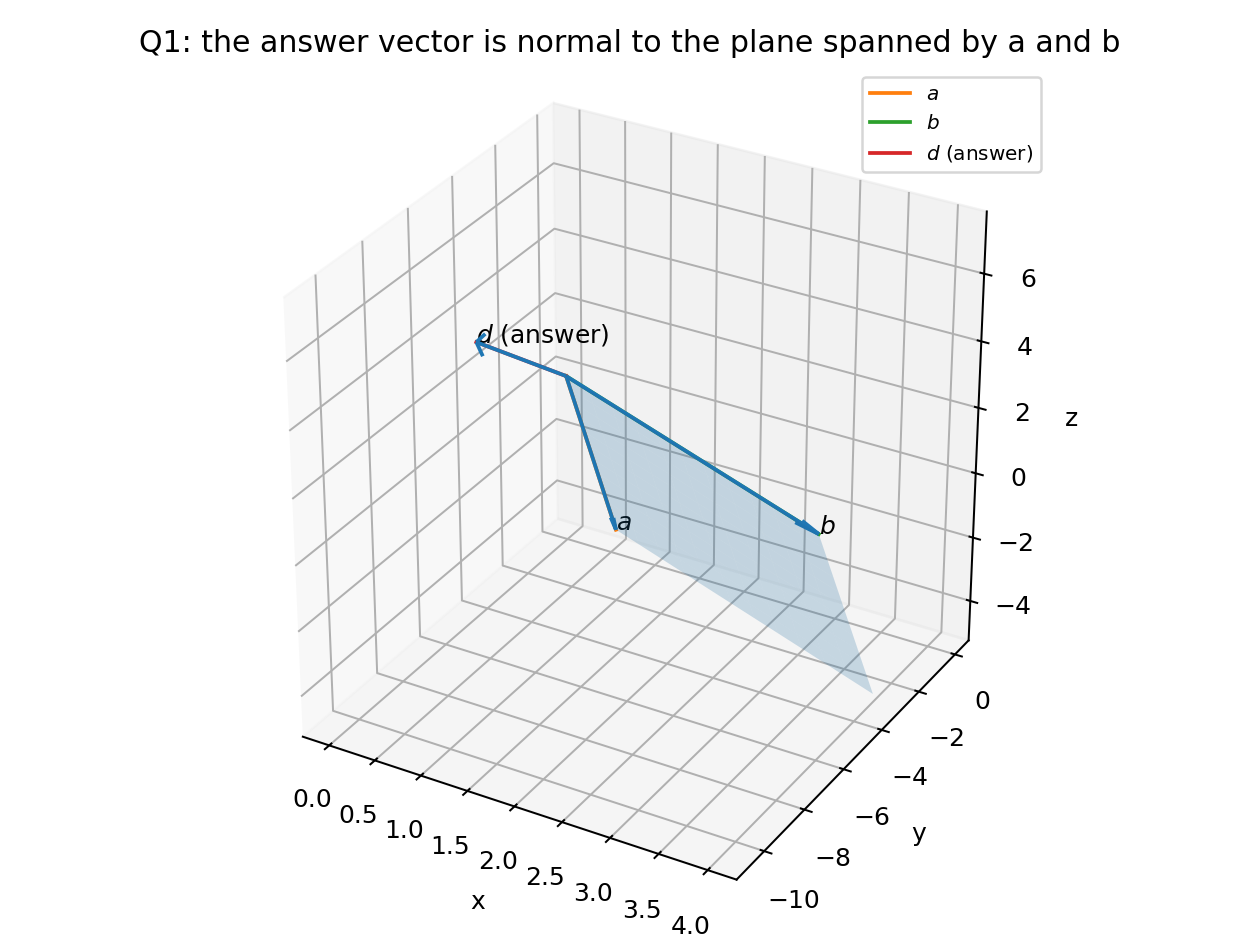
\includegraphics[width=0.96\linewidth]{figs/Q01_3D.png}\end{figure}
\par\smallskip
\noindent\textbf{Code reference -- plotting and numerical verification}
\par\noindent\fbox{\parbox{\dimexpr\linewidth-2\fboxsep-2\fboxrule\relax}{\centering\texttt{codes/Q01.py}}}
\par\smallskip

\item[\textbf{1.2.5}] Let $\vec a=\myvec{1\\4\\2}$, $\vec b=\myvec{3\\-2\\7}$ and $\vec c=\myvec{2\\-1\\4}$. Find $\vec d$ perpendicular to both $\vec a,\vec b$ with $\vec c\cdot\vec d=27$.
\solution The required direction is $\vec a\times\vec b=(32,-1,-14)^T$. Set $\vec d=t(32,-1,-14)^T$. Since $\vec c\cdot(\vec a\times\vec b)=9$, the constraint gives $9t=27$, hence
\[
\vec d=\myvec{96\\-3\\-42}.
\]
\begin{figure}[H]\centering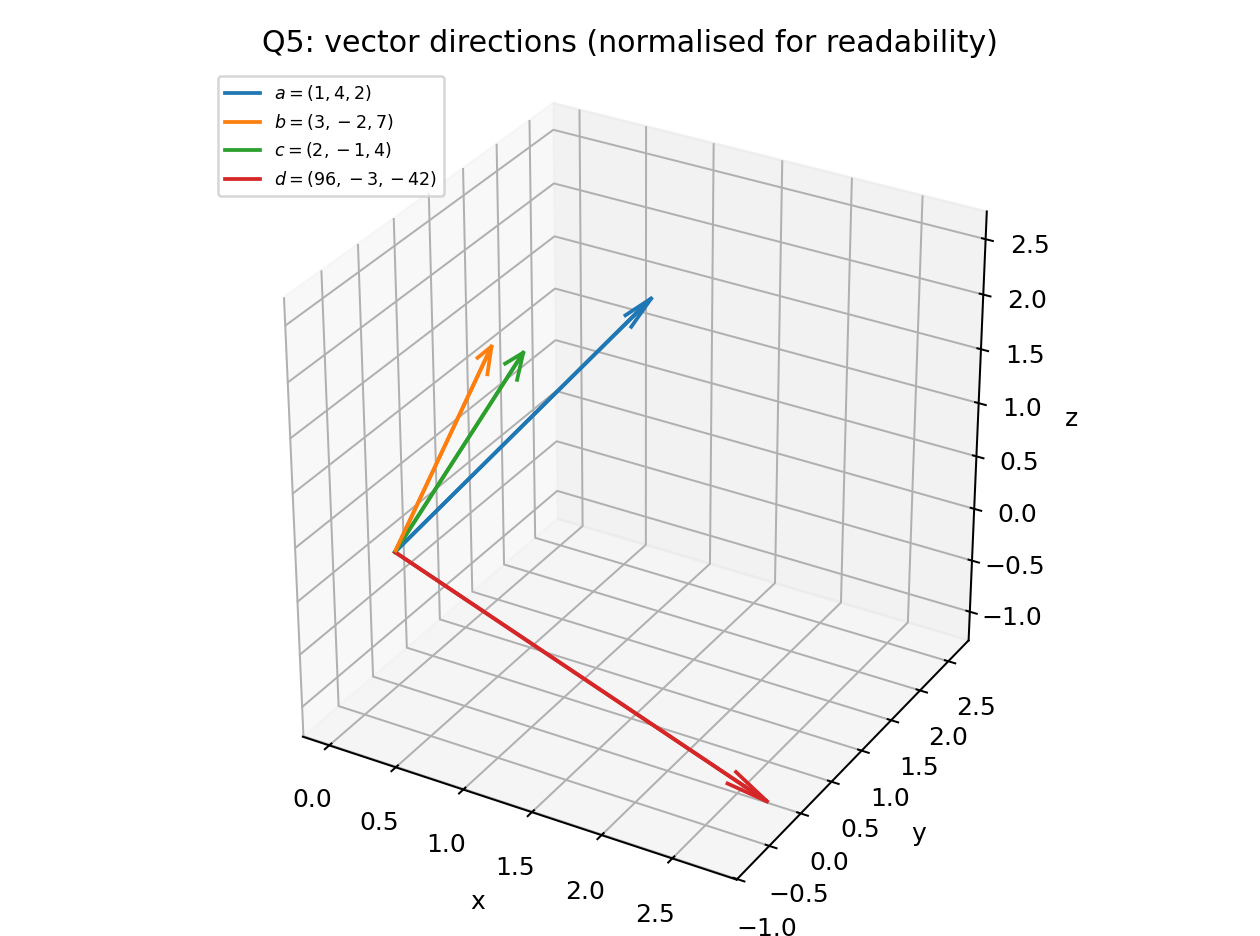
\includegraphics[width=0.96\linewidth]{figs/Q05_3D.png}\end{figure}
\par\smallskip
\noindent\textbf{Code reference -- plotting and numerical verification}
\par\noindent\fbox{\parbox{\dimexpr\linewidth-2\fboxsep-2\fboxrule\relax}{\centering\texttt{codes/Q05.py}}}
\par\smallskip

\item[\textbf{1.2.6}] Find the shortest distance between $\vec r=(1,2,3)+\lambda(2,3,4)$ and $\vec r=(2,4,5)+\mu(4,6,8)$.
\solution The direction vectors are parallel, since $(4,6,8)=2(2,3,4)$. For parallel lines the distance is the perpendicular distance from one point to the other line:
\[
d=\frac{\norm{(B-A)\times\vec v}}{\norm{\vec v}},\quad B-A=(1,2,2),\quad \vec v=(2,3,4).
\]
Here $(B-A)\times\vec v=(2,0,-1)$, so
\[
d=\frac{\sqrt5}{\sqrt{29}}.
\]
\begin{figure}[H]\centering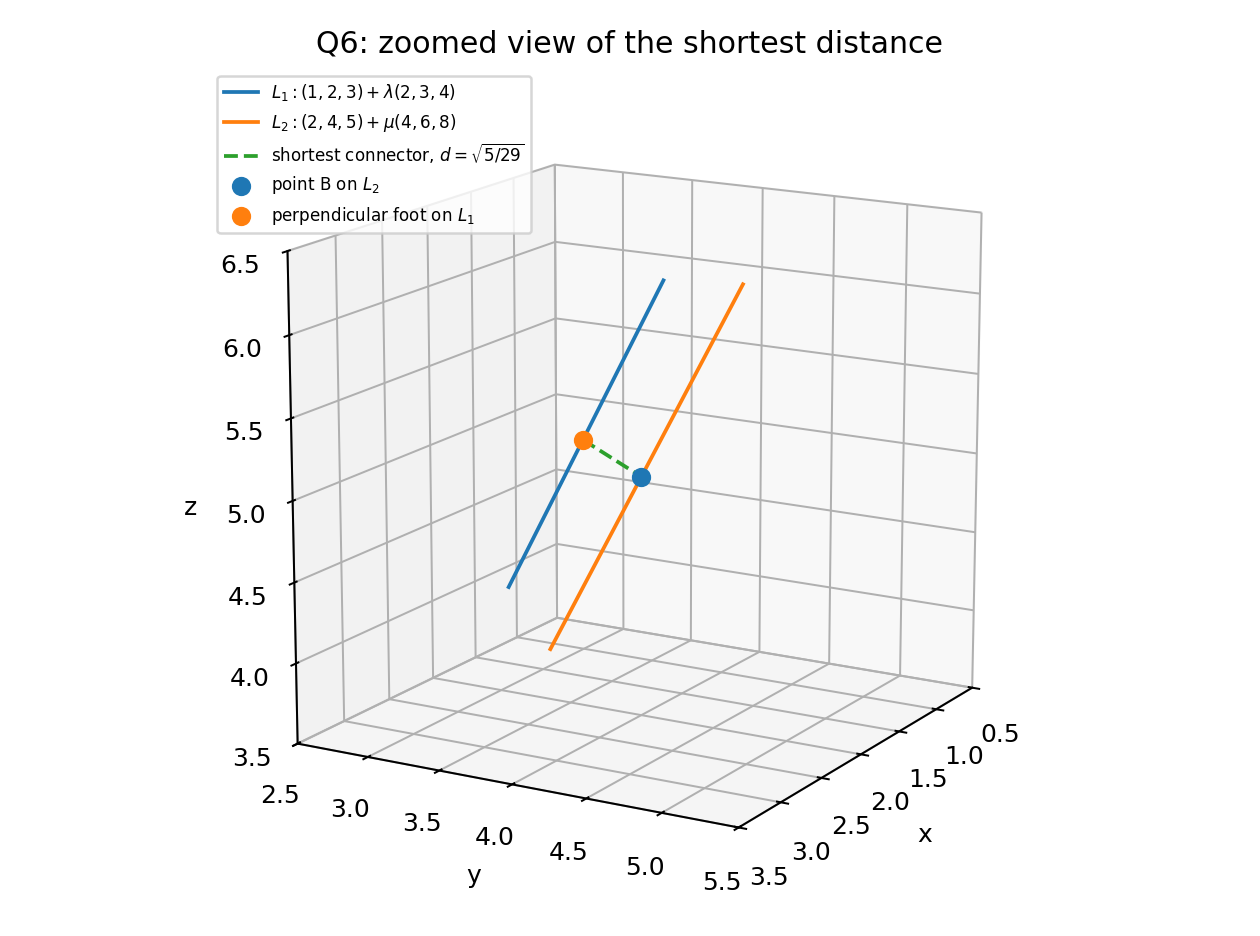
\includegraphics[width=0.96\linewidth]{figs/Q06_3D.png}\end{figure}
\par\smallskip
\noindent\textbf{Code reference -- plotting and numerical verification}
\par\noindent\fbox{\parbox{\dimexpr\linewidth-2\fboxsep-2\fboxrule\relax}{\centering\texttt{codes/Q06.py}}}
\par\smallskip

\end{enumerate}

\paragraph*{Lines and planes}
\begin{enumerate}[label={},leftmargin=0pt,itemsep=9pt]
\item[\textbf{1.2.10}] Find the plane through the intersection of $2x+y-z=3$ and $5x-3y+4z+9=0$ that is parallel to $\frac{x-1}{2}=\frac{y-3}{-4}=\frac{5-z}{-5}$.
\solution A plane through the intersection has equation
\[
(2x+y-z-3)+\lambda(5x-3y+4z+9)=0.
\]
The line direction is $(2,-4,5)$. Its dot product with the plane normal $(2+5\lambda,1-3\lambda,-1+4\lambda)$ must vanish:
\[
2(2+5\lambda)-4(1-3\lambda)+5(-1+4\lambda)=0,
\]
so $\lambda=5/42$. Multiplying by 42 and simplifying gives
\[
109x+27y-22z-81=0.
\]
\begin{figure}[H]\centering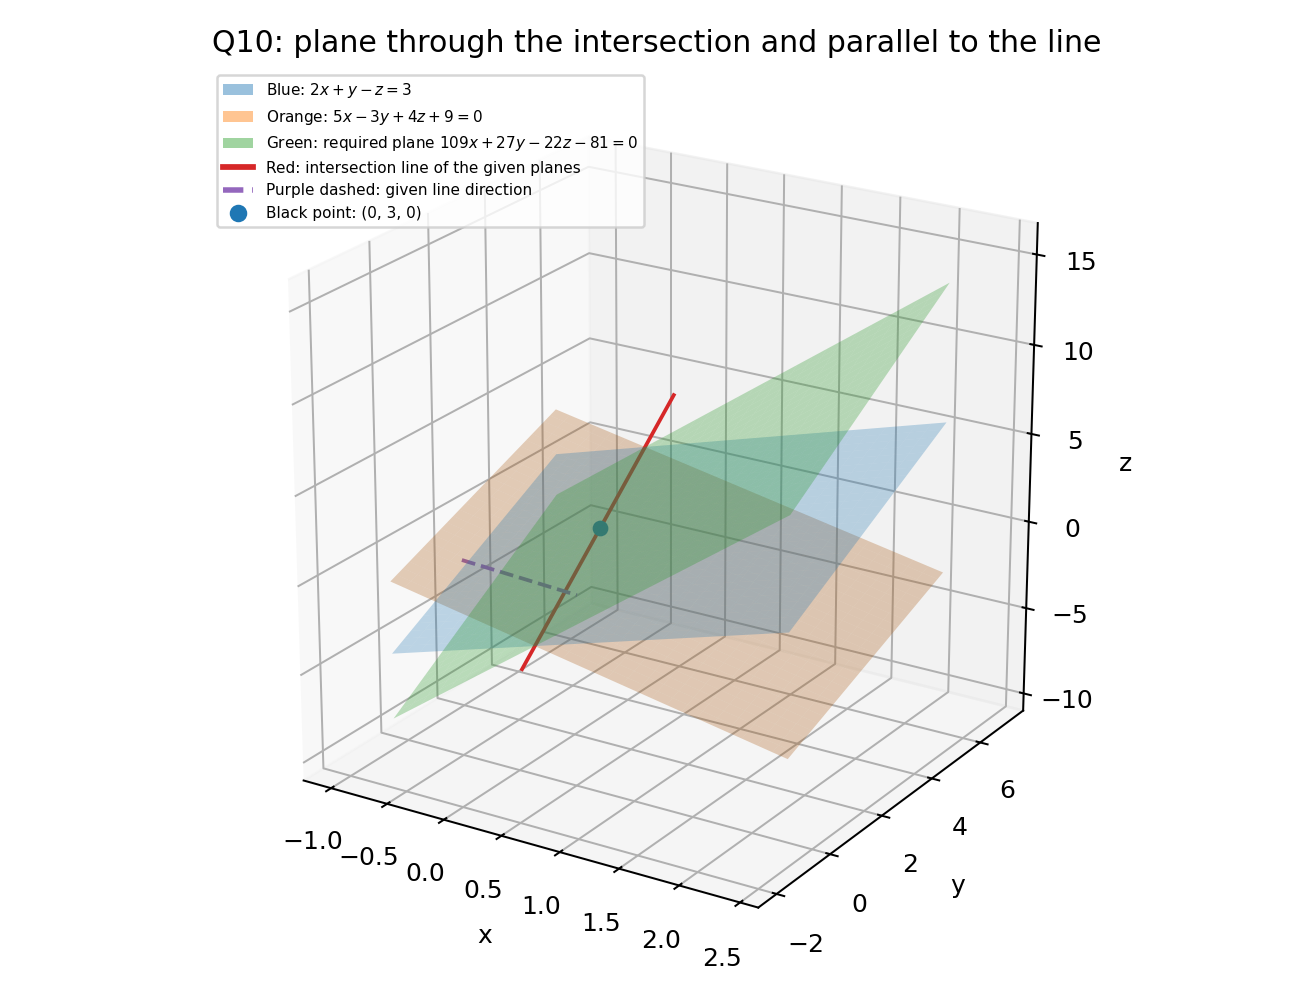
\includegraphics[width=0.96\linewidth]{figs/Q10_3D.png}\end{figure}
\par\smallskip
\noindent\textbf{Code reference -- plotting and numerical verification}
\par\noindent\fbox{\parbox{\dimexpr\linewidth-2\fboxsep-2\fboxrule\relax}{\centering\texttt{codes/Q10.py}}}
\par\smallskip

\item[\textbf{1.2.15}] Find where the line through $A(3,4,1)$ and $B(5,1,6)$ meets the plane through $P(2,1,2)$, $Q(3,1,0)$ and $R(4,-2,1)$.
\solution A normal to the plane is $(Q-P)\times(R-P)=(1,0,-2)\times(2,-3,-1)\propto(2,1,1)$. Thus the plane is $2x+y+z=7$. The line is $(3,4,1)+t(2,-3,5)$. Substitution into the plane yields $4+6t=0$, so $t=-2/3$. The intersection is
\[
\left(\frac53,6,-\frac73\right).
\]
\begin{figure}[H]\centering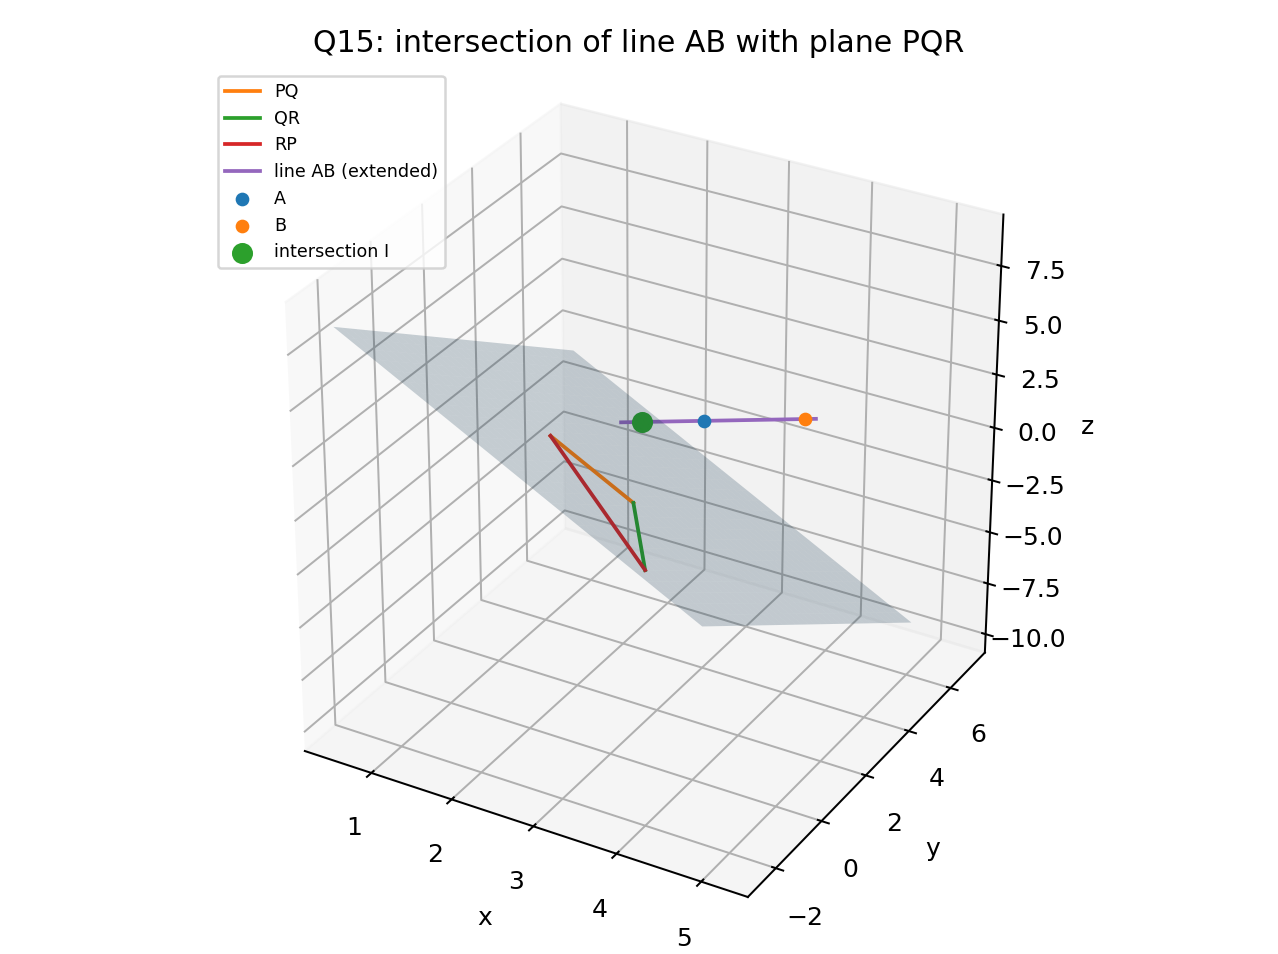
\includegraphics[width=0.96\linewidth]{figs/Q15_3D.png}\end{figure}
\par\smallskip
\noindent\textbf{Code reference -- plotting and numerical verification}
\par\noindent\fbox{\parbox{\dimexpr\linewidth-2\fboxsep-2\fboxrule\relax}{\centering\texttt{codes/Q15.py}}}
\par\smallskip
\end{enumerate}

\paragraph*{Differential equations}
\begin{enumerate}[label={},leftmargin=0pt,itemsep=9pt]
\item[\textbf{1.2.20}] Find the integrating factor of $x\log x\,\frac{dy}{dx}+y=2\log x$.
\solution In standard form,
\[
y'+\frac{1}{x\log x}y=\frac2x.
\]
Thus the integrating factor is
\[
\exp\!\left(\int\frac{dx}{x\log x}\right)=\exp(\log|\log x|).
\]
On a domain where $\log x>0$, this is $\log x$ (more generally the factor can be taken as $|\log x|$ on an interval not crossing $x=1$).

\item[\textbf{1.2.21}] Find the differential equation of the family $(x-h)^2+(y-k)^2=r^2$, where $h,k$ are arbitrary constants and $r$ is fixed.
\solution Differentiate once:
\[
(x-h)+(y-k)y'=0.
\]
Differentiate again: $1+(y')^2+(y-k)y''=0$, giving $y-k=-(1+(y')^2)/y''$. Substitute this and $x-h=-(y-k)y'$ into the original circle equation. Then
\[
\frac{(1+(y')^2)^3}{(y'')^2}=r^2,
\quad(1+(y')^2)^3=r^2(y'')^2.
\]

\item[\textbf{1.2.22}] Show that $(x-y)\frac{dy}{dx}=x+2y$ is homogeneous and solve it.
\solution The derivative is a ratio of homogeneous first-degree expressions. Put $y=vx$, so $y'=v+xv'$. Substitution gives
\[
x\frac{dv}{dx}=\frac{1+v+v^2}{1-v},\qquad
\frac{1-v}{1+v+v^2}\,dv=\frac{dx}{x}.
\]
Integrating,
\[
-\frac12\ln(v^2+v+1)+\sqrt3\tan^{-1}\!\left(\frac{2v+1}{\sqrt3}\right)=\ln|x|+C.
\]
Using $v=y/x$ gives the implicit solution
\[
-\tfrac12\ln\!\left(\frac{y^2}{x^2}+\frac yx+1\right)+\sqrt3\tan^{-1}\!\left(\frac{2y/x+1}{\sqrt3}\right)=\ln|x|+C.
\]

\item[\textbf{1.2.24}] Find the particular solution of $y'+y\tan x=3x^2+x^3\tan x$, given $y=0$ at $x=\pi/3$ and $x\ne\pi/2$.
\solution The integrating factor is $e^{\int\tan x\,dx}=\sec x$. Multiplication gives
\[
\frac{d}{dx}(y\sec x)=3x^2\sec x+x^3\sec x\tan x=\frac{d}{dx}(x^3\sec x).
\]
So $y\sec x=x^3\sec x+C$ and $y=x^3+C\cos x$. From $y(\pi/3)=0$, $C=-2\pi^3/27$. Therefore
\[
y=x^3-\frac{2\pi^3}{27}\cos x.
\]
\par\smallskip
\noindent\textbf{Code reference -- numerical verification}
\par\noindent\fbox{\parbox{\dimexpr\linewidth-2\fboxsep-2\fboxrule\relax}{\centering\texttt{codes/Q24.py}}}
\par\smallskip

\item[\textbf{1.2.25}] If $y=\log\left(\frac{x}{a+bx}\right)^x$, prove that $x^3y''=(xy'-y)^2$.
\solution Interpret the expression as $y=x\log\left(\frac{x}{a+bx}\right)$. Then
\[
y'=\log\left(\frac{x}{a+bx}\right)+\frac{a}{a+bx},\qquad
 y''=\frac{a^2}{x(a+bx)^2}.
\]
Thus $xy'-y=ax/(a+bx)$ and
\[
x^3y''=\frac{a^2x^2}{(a+bx)^2}=(xy'-y)^2.
\]
\end{enumerate}



\paragraph*{Matrices and determinants}
\begin{enumerate}[label={},leftmargin=0pt,itemsep=9pt]
\item[\textbf{1.2.28}] If $A=\myvec{\cos\theta&\sin\theta\\\sin\theta&\cos\theta}$, find $\det(A^n)$ for natural $n$.
\solution Determinants are multiplicative, so $\det(A^n)=(\det A)^n$. Now $\det A=\cos^2\theta-\sin^2\theta=\cos2\theta$. Thus
\[
\det(A^n)=(\cos2\theta)^n.
\]

\item[\textbf{1.2.30}] Find the inverse of $\myvec{0&1&2\\1&2&3\\3&1&0}$ using elementary row operations.
\solution Augment the matrix by $I$ and row-reduce to $[I\mid A^{-1}]$. The determinant is $-1$, so the matrix is invertible. The result is
\[
A^{-1}=\myvec{3&-2&1\\-9&6&-2\\5&-3&1}.
\]
The product check $AA^{-1}=I$ is carried out in code.
\par\smallskip
\noindent\textbf{Code reference -- numerical verification}
\par\noindent\fbox{\parbox{\dimexpr\linewidth-2\fboxsep-2\fboxrule\relax}{\centering\texttt{codes/Q30.py}}}
\par\smallskip

\item[\textbf{1.2.36}] If $a+b+c\ne0$ and $\mydet{a&b&c\\b&c&a\\c&a&b}=0$, prove that $a=b=c$.
\solution Expanding and factorising the determinant gives
\[
-(a+b+c)(a^2+b^2+c^2-ab-bc-ca)=0.
\]
The first factor is nonzero by assumption, so $a^2+b^2+c^2-ab-bc-ca=0$. But
\[
a^2+b^2+c^2-ab-bc-ca=\tfrac12[(a-b)^2+(b-c)^2+(c-a)^2].
\]
Each square must be zero, hence $a=b=c$.

\item[\textbf{1.2.37}] A trust receives Rs. 30,000 per month. Half is spent on care, and 2\% of the amount spent is collected from beneficiaries. The unspent balance is deposited in a bank. Find the monthly interest rate needed for total monthly income of Rs. 1800.
\solution Let $u$ be the monthly contribution collected from beneficiaries and $v$ the bank interest. Half of Rs. $30,000$ is spent, so
\[
u=0.02(15000)=300.
\]
The total monthly income is Rs. $1800$, so
\[
u+v=1800,\qquad u=300.
\]
Write this system as an augmented matrix:
\[
\left[\begin{array}{cc|c}1&1&1800\\1&0&300\end{array}\right]
\xrightarrow{R_2\leftarrow R_2-R_1}
\left[\begin{array}{cc|c}1&1&1800\\0&-1&-1500\end{array}\right]
\xrightarrow{R_2\leftarrow -R_2}
\left[\begin{array}{cc|c}1&1&1800\\0&1&1500\end{array}\right].
\]
Eliminate $v$ from the first row:
\[
R_1\leftarrow R_1-R_2:\qquad
\left[\begin{array}{cc|c}1&0&300\\0&1&1500\end{array}\right].
\]
Thus $u=300$ and $v=1500$. The deposit is Rs. $15000$, therefore
\[
r=\frac{1500}{15000}\times100\%=10\%\text{ per month}.
\]
\par\smallskip
\noindent\textbf{Code reference -- numerical verification}
\par\noindent\fbox{\parbox{\dimexpr\linewidth-2\fboxsep-2\fboxrule\relax}{\centering\texttt{codes/Q37.py}}}
\par\smallskip

\end{enumerate}

\paragraph*{Integration and area}
\begin{enumerate}[label={},leftmargin=0pt,itemsep=9pt]
\item[\textbf{1.2.38}] Evaluate $\displaystyle I=\int_0^{\pi/2}\frac{\cos^2x}{1+3\sin^2x}\,dx$.
\solution Let $t=\tan x$. Then $dx=dt/(1+t^2)$ and the integral becomes
\[
I=\int_0^\infty\frac{dt}{(1+t^2)(1+4t^2)}=\int_0^\infty\left[-\frac1{3(1+t^2)}+\frac4{3(1+4t^2)}\right]dt.
\]
Evaluating the arctangent limits gives $I=-\pi/6+\pi/3=\pi/6$.

\item[\textbf{1.2.39}] Evaluate $\displaystyle\int_0^{\pi/4}\frac{\sin x+\cos x}{3+\sin2x}\,dx$.
\solution Set $u=\sin x-\cos x$, so $du=(\sin x+\cos x)dx$ and $\sin2x=1-u^2$. The limits become $u=-1$ and $u=0$. Hence
\[
I=\int_{-1}^{0}\frac{du}{4-u^2}=\left[\frac14\ln\left|\frac{2+u}{2-u}\right|\right]_{-1}^{0}=\frac14\ln3.
\]

\item[\textbf{1.2.40}] Evaluate $\displaystyle\int\frac{\sin x-x\cos x}{x(x+\sin x)}\,dx$.
\solution Since
\[
\frac{d}{dx}\ln\left|\frac{x}{x+\sin x}\right|=\frac{\sin x-x\cos x}{x(x+\sin x)},
\]
the integral is $\ln\left|\frac{x}{x+\sin x}\right|+C$.

\item[\textbf{1.2.41}] Evaluate $\displaystyle\int\frac{x^3}{(x-1)(x^2+1)}\,dx$.
\solution Polynomial division and partial fractions give
\[
\frac{x^3}{(x-1)(x^2+1)}=1+\frac1{2(x-1)}+\frac{x-1}{2(x^2+1)}.
\]
Therefore
\[
x+\frac12\ln|x-1|+\frac14\ln(x^2+1)-\frac12\tan^{-1}x+C.
\]

\item[\textbf{1.2.42}] Find $\displaystyle\int\frac{x\,dx}{1+x\tan x}$.
\solution Rewrite the integrand as $x\cos x/(\cos x+x\sin x)$. Since $d(\cos x+x\sin x)/dx=x\cos x$,
\[
\int\frac{x\,dx}{1+x\tan x}=\ln|\cos x+x\sin x|+C.
\]

\item[\textbf{1.2.43}] Evaluate $\displaystyle\int\frac{x^4}{(x-1)(x^2+1)}\,dx$.
\solution Division gives $x^4/[(x-1)(x^2+1)]=x+1+1/[(x-1)(x^2+1)]$. Decompose the last term as
\[
\frac1{(x-1)(x^2+1)}=\frac1{2(x-1)}-\frac{x+1}{2(x^2+1)}.
\]
Thus
\[
\frac{x^2}{2}+x+\frac12\ln|x-1|-\frac14\ln(x^2+1)-\frac12\tan^{-1}x+C.
\]

\item[\textbf{1.2.44}] Evaluate $\displaystyle\int_0^{\pi/2}\frac{5\sin x+3\cos x}{\sin x+\cos x}\,dx$.
\solution Write the numerator as $4(\sin x+\cos x)+(\sin x-\cos x)$. Then
\[
I=4\int_0^{\pi/2}dx-\left[\ln(\sin x+\cos x)\right]_0^{\pi/2}=2\pi.
\]

\item[\textbf{1.2.45}] Find $\displaystyle\int\left[\log(\log x)+\frac1{(\log x)^2}\right]dx$.
\solution Differentiate $x\log(\log x)-x/\log x$ to check that it equals the integrand. Hence
\[
x\log(\log x)-\frac{x}{\log x}+C,\qquad x>1\text{ for a real-valued }\log(\log x).
\]

\item[\textbf{1.2.46}] If the area bounded by $y^2=16ax$ and $y=4mx$ is $a^2/2$, find $m$.
\solution Use the upper branch $y=4\sqrt{ax}$. At an intersection with $y=4mx$,
\[
4\sqrt{ax}=4mx\quad\Longrightarrow\quad x=0\quad\text{or}\quad x=\frac{a}{m^2}.
\]
For positive slope, the area is the integral of the parabola minus the line:
\begin{align*}
A&=\int_0^{a/m^2}\left(4\sqrt{ax}-4mx\right)\,dx\\
 &=\left[\frac{8\sqrt a}{3}x^{3/2}-2mx^2\right]_0^{a/m^2}\\
 &=\frac{8a^2}{3m^3}-\frac{2a^2}{m^3}=\frac{2a^2}{3m^3}.
\end{align*}
Set the result equal to the given area:
\[
\frac{2a^2}{3m^3}=\frac{a^2}{2}\quad\Longrightarrow\quad4=3m^3\quad\Longrightarrow\quad m=\sqrt[3]{\frac43}.
\]
The graph uses $a=1$ for visibility; the value of $m$ is independent of that scale.
\begin{figure}[H]\centering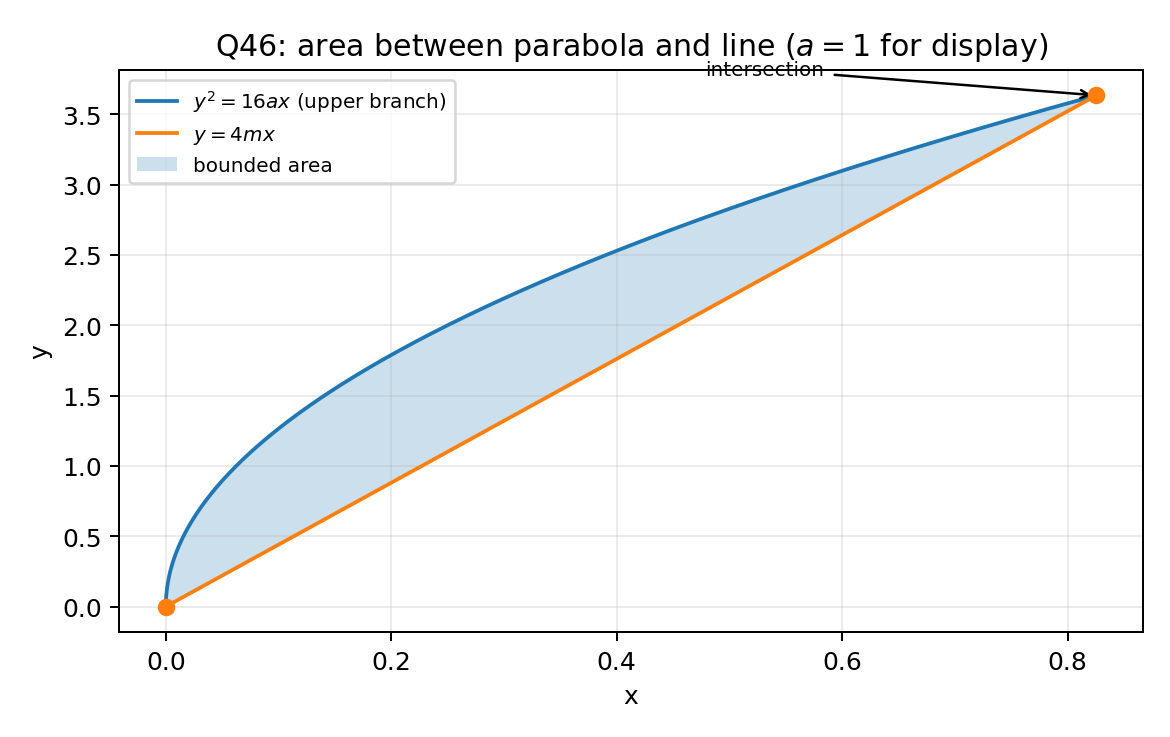
\includegraphics[width=0.92\linewidth]{figs/Q46_ParabolaArea.png}\end{figure}
\par\smallskip
\noindent\textbf{Code reference -- plotting}
\par\noindent\fbox{\parbox{\dimexpr\linewidth-2\fboxsep-2\fboxrule\relax}{\centering\texttt{codes/Q46.py}}}
\par\smallskip

\item[\textbf{1.2.47}] Find the area of $\{(x,y):x^2+y^2\le4,\;x+y\ge2\}$ by integration.
\solution The chord $x+y=2$ meets the circle at $(0,2)$ and $(2,0)$. For $0\le x\le2$, the upper circle boundary is $y=\sqrt{4-x^2}$ and the line is $y=2-x$. Therefore
\begin{align*}
A&=\int_0^2\left(\sqrt{4-x^2}-(2-x)\right)dx\\
 &=\underbrace{\int_0^2\sqrt{4-x^2}\,dx}_{\text{quarter-circle area }=\pi}
 -\underbrace{\int_0^2(2-x)\,dx}_{\text{triangle area }=2}\\
 &=\pi-2\quad\text{square units}.
\end{align*}
The graph shades the circular segment above the chord.
\begin{figure}[H]\centering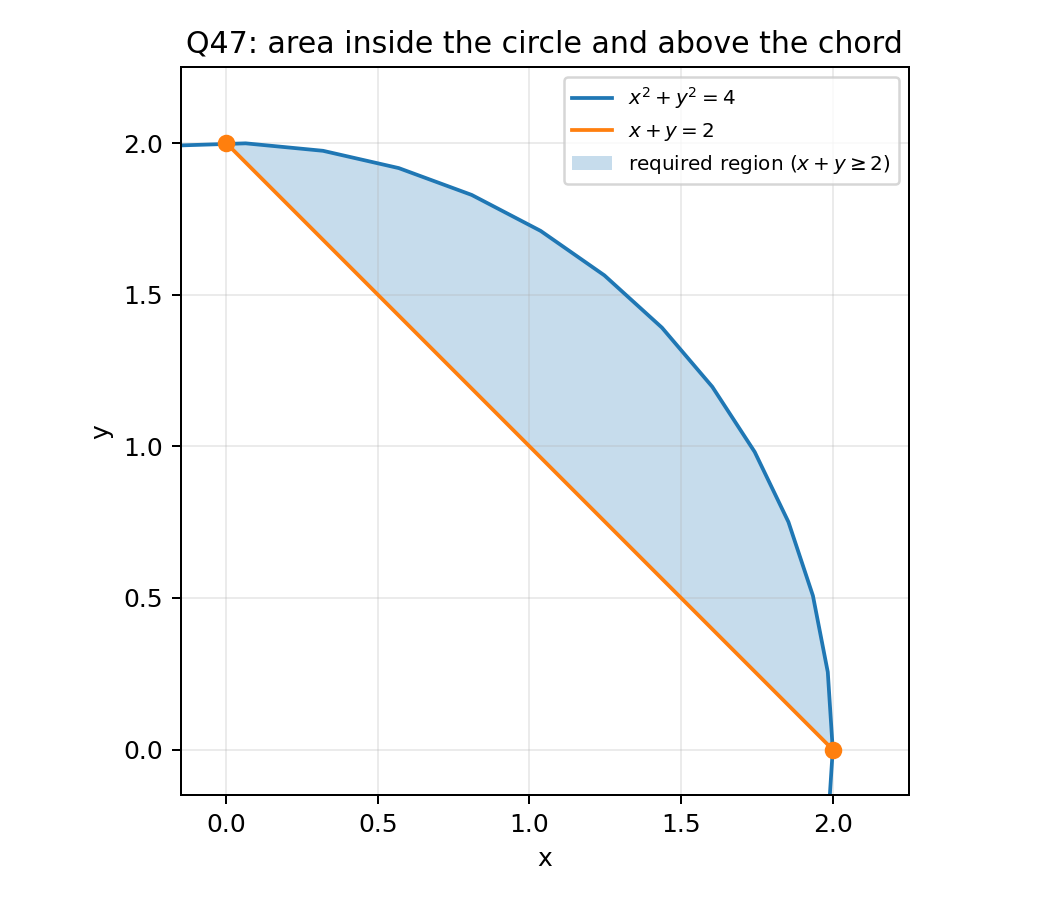
\includegraphics[width=0.92\linewidth]{figs/Q47_CircleSegment.png}\end{figure}
\par\smallskip
\noindent\textbf{Code reference -- plotting}
\par\noindent\fbox{\parbox{\dimexpr\linewidth-2\fboxsep-2\fboxrule\relax}{\centering\texttt{codes/Q47.py}}}
\par\smallskip
\end{enumerate}

\paragraph*{Functions and relations}
\begin{enumerate}[label={},leftmargin=0pt,itemsep=9pt]
\item[\textbf{1.2.48}] Discuss continuity and differentiability of $f(x)=|x|+|x-1|$ on $(-1,2)$.
\solution First split the absolute values at $x=0$ and $x=1$:
\[
f(x)=\begin{cases}
1-2x,&-1<x<0,\\
1,&0\le x<1,\\
2x-1,&1\le x<2.
\end{cases}
\]
\textbf{Continuity.} At $x=0$, the left limit, right limit and function value are all $1$. The same is true at $x=1$. Each branch is continuous on its interval; hence $f$ is continuous throughout $(-1,2)$.

\textbf{Differentiability at $x=0$.} The left-hand slope is $-2$ and the right-hand slope is $0$:
\[
f'_-(0)=-2\ne0=f'_+(0).
\]
Thus $f$ is not differentiable at $0$.

\textbf{Differentiability at $x=1$.} The left-hand slope is $0$ and the right-hand slope is $2$:
\[
f'_-(1)=0\ne2=f'_+(1).
\]
Thus $f$ is not differentiable at $1$. At other points the function is linear and differentiable. The plot shows these one-sided slopes: differentiability requires equal one-sided slopes, and the two corners fail that test.
\begin{figure}[H]\centering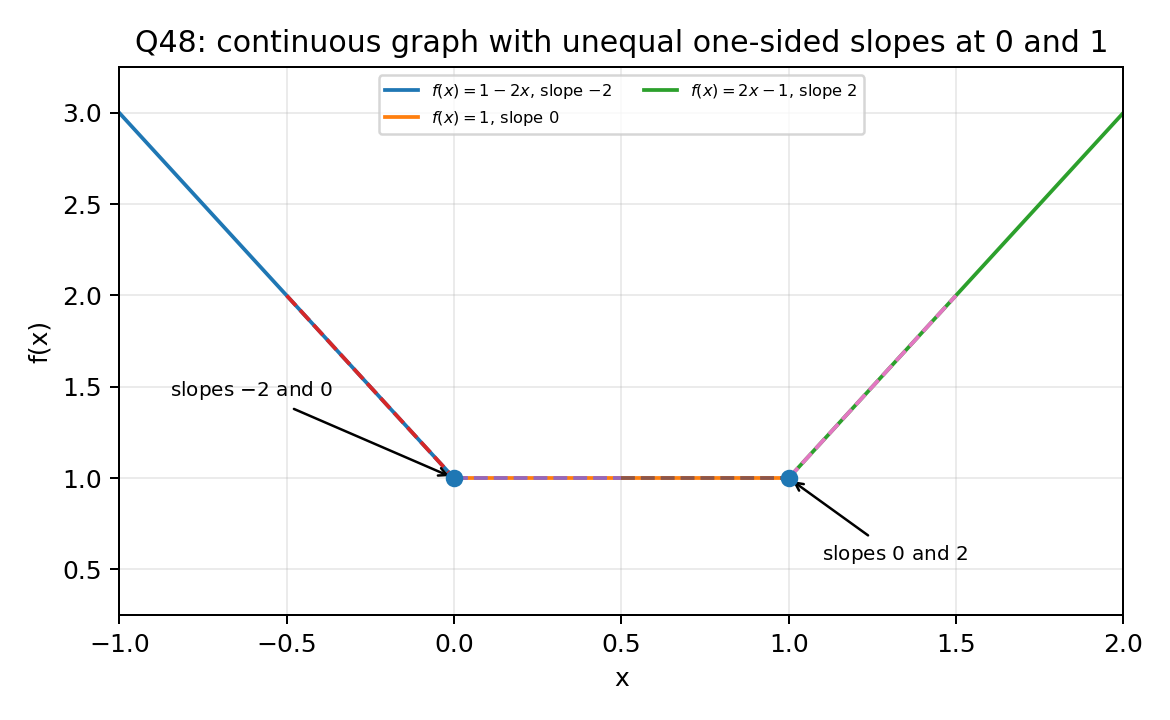
\includegraphics[width=0.92\linewidth]{figs/Q48_Differentiability.png}\end{figure}
\par\smallskip
\noindent\textbf{Code reference -- plotting and slope verification}
\par\noindent\fbox{\parbox{\dimexpr\linewidth-2\fboxsep-2\fboxrule\relax}{\centering\texttt{codes/Q48.py}}}
\par\smallskip

\item[\textbf{1.2.49}] On $\mathbb R$, define $(a,b)\in R$ when $a-b+\sqrt3$ is irrational. Determine whether $R$ is reflexive, symmetric and transitive.
\solution We test each property separately.

\textbf{1. Reflexive.} Reflexivity requires $(a,a)\in R$ for every real $a$. Substituting $b=a$ gives
\[
a-a+\sqrt3=\sqrt3,
\]
which is irrational. Therefore $R$ is reflexive.

\textbf{2. Symmetric.} Symmetry requires $(a,b)\in R$ to imply $(b,a)\in R$. Choose $a=\sqrt3$ and $b=0$. Then
\[
a-b+\sqrt3=2\sqrt3
\]
is irrational, so $(a,b)\in R$. Reversing the pair gives
\[
b-a+\sqrt3=0,
\]
which is rational, so $(b,a)\notin R$. Hence $R$ is not symmetric.

\textbf{3. Transitive.} Transitivity requires $(a,b),(b,c)\in R$ to imply $(a,c)\in R$. Choose $a=\sqrt3$, $b=0$, and $c=2\sqrt3$. Then
\[
a-b+\sqrt3=2\sqrt3,\qquad b-c+\sqrt3=-\sqrt3,
\]
both irrational, so $(a,b),(b,c)\in R$. However,
\[
a-c+\sqrt3=\sqrt3-2\sqrt3+\sqrt3=0,
\]
which is rational. Thus $(a,c)\notin R$, and $R$ is not transitive.

\textbf{Conclusion.} $R\text{ is reflexive, but neither symmetric nor transitive.}$

\item[\textbf{1.2.50}] On $\mathbb R\times\mathbb R$, define $(a,b)*(c,d)=(a+c,b+d)$. Prove commutativity and associativity, and find the identity and the inverse of $(3,-5)$.
\solution Addition of real components is commutative and associative, so $*$ has both properties. Its identity is $(0,0)$, since $(a,b)*(0,0)=(a,b)$. The inverse of $(3,-5)$ is $(-3,5)$.

\item[\textbf{1.2.51}] On $\{0,1,2,3,4,5,6\}$ define $a*b=a+b$ if $a+b<7$, and $a*b=a+b-7$ otherwise. Give the operation table and show that 0 is the identity and $7-a$ is the inverse for nonzero $a$.
\solution This is addition modulo 7. Its table is
\[
\begin{array}{c|rrrrrrr}
* &0&1&2&3&4&5&6\\\hline
0&0&1&2&3&4&5&6\\
1&1&2&3&4&5&6&0\\
2&2&3&4&5&6&0&1\\
3&3&4&5&6&0&1&2\\
4&4&5&6&0&1&2&3\\
5&5&6&0&1&2&3&4\\
6&6&0&1&2&3&4&5
\end{array}
\]
Row and column 0 reproduce every element, hence 0 is the identity. For each $a=1,\ldots,6$, $a+(7-a)=7\equiv0\pmod7$, so $7-a$ is its inverse.

\item[\textbf{1.2.52}] Find any point of discontinuity of $f(x)=x-|x-x^2|$, $x\in[-1,1]$.
\solution On $[-1,1]$, $x-x^2=x(1-x)$, whose sign changes only at 0. Thus
\[
f(x)=\begin{cases}2x-x^2,&-1\le x\le0,\\x^2,&0\le x\le1.\end{cases}
\]
Both pieces take value 0 at $x=0$ and meet continuously. The endpoints are also included continuously. Therefore there are \text{no points of discontinuity}.
\begin{figure}[H]\centering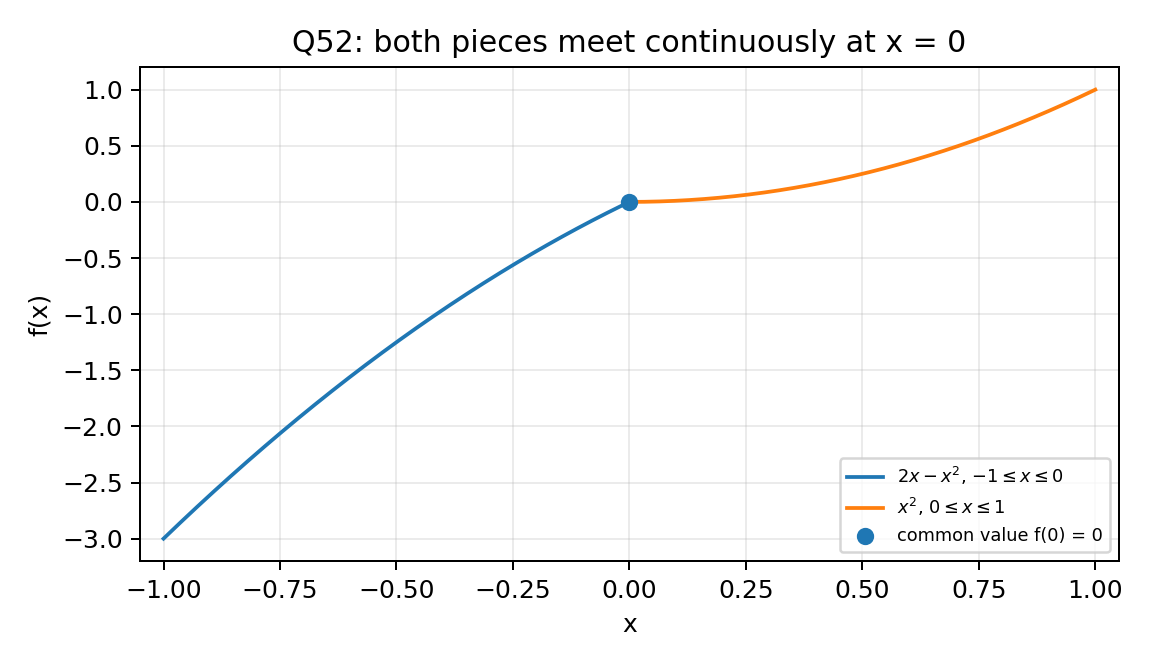
\includegraphics[width=0.92\linewidth]{figs/Q52_Continuity.png}\end{figure}
\par\smallskip
\noindent\textbf{Code reference -- plotting}
\par\noindent\fbox{\parbox{\dimexpr\linewidth-2\fboxsep-2\fboxrule\relax}{\centering\texttt{codes/Q52.py}}}
\par\smallskip
\end{enumerate}

\paragraph*{Probability}
\begin{enumerate}[label={},leftmargin=0pt,itemsep=9pt]
\item[\textbf{1.2.53}] A man steps forward with probability $0.4$ and backward with probability $0.6$. Find the probability that after 5 steps he is one step away from his starting point.
\solution Let $k$ be the number of forward steps. The net displacement after five steps is
\[
D=k-(5-k)=2k-5.
\]
One step away means $D=+1$ or $D=-1$. These occur when $k=3$ or $k=2$, respectively.

\textbf{Step 1: Net displacement $+1$.} Three steps are forward and two backward, so the binomial formula gives
\begin{align*}
P(D=1)&=\binom53(0.4)^3(0.6)^2\\
&=10(0.064)(0.36)=0.2304.
\end{align*}

\textbf{Step 2: Net displacement $-1$.} Two steps are forward and three backward:
\begin{align*}
P(D=-1)&=\binom52(0.4)^2(0.6)^3\\
&=10(0.16)(0.216)=0.3456.
\end{align*}

\textbf{Step 3: Add the disjoint events.}
\[
P(|D|=1)=P(D=1)+P(D=-1)=0.2304+0.3456=0.576.
\]

\textbf{Generating function / $Z$-transform.} For one step, the Laurent probability generating function is $G(z)=0.4z+0.6z^{-1}$. For five independent steps,
\[
G_5(z)=(0.4z+0.6z^{-1})^5
=\sum_{k=0}^5\binom5k(0.4)^k(0.6)^{5-k}z^{2k-5}.
\]
The coefficient of $z^1$ is $0.2304$ and the coefficient of $z^{-1}$ is $0.3456$. Their sum is the required probability. The plot shows the theoretical PMF for every possible displacement.
\begin{figure}[H]\centering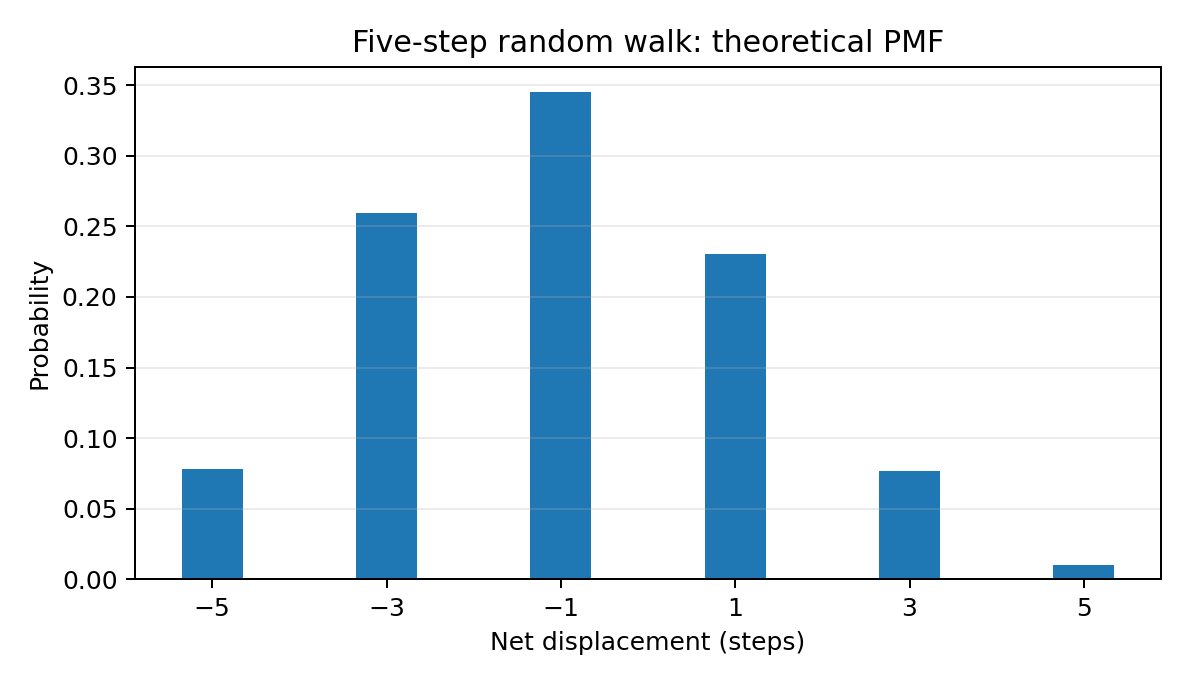
\includegraphics[width=0.92\linewidth]{figs/Q53_WalkPMF.png}\end{figure}
\par\smallskip
\noindent\textbf{Code reference -- plotting and numerical verification}
\par\noindent\fbox{\parbox{\dimexpr\linewidth-2\fboxsep-2\fboxrule\relax}{\centering\texttt{codes/Q53.py}}}
\par\smallskip

\item[\textbf{1.2.54}] A girl throws a die. If it shows 1 or 2, she tosses a coin three times; otherwise she tosses it once. Given that exactly one tail was obtained, find the probability that the die showed 3, 4, 5 or 6.
\solution Let $A$ mean that the die shows 1 or 2, $B$ mean that it shows 3, 4, 5 or 6, and $E$ mean that exactly one tail is observed.

\textbf{Step 1: Find the prior probabilities.}
\[
P(A)=\frac26=\frac13,\qquad P(B)=\frac46=\frac23.
\]

\textbf{Step 2: Find the likelihood of $E$.} If $A$ occurs, three fair coin tosses are made. Exactly one tail can occur in $\binom31$ of the 8 equally likely outcomes:
\[
P(E\mid A)=\binom31\left(\frac12\right)^3=\frac38.
\]
If $B$ occurs, only one coin toss is made, so
\[
P(E\mid B)=\frac12.
\]

\textbf{Step 3: Calculate $P(E)$ by total probability.}
\begin{align*}
P(E)&=P(E\mid A)P(A)+P(E\mid B)P(B)\\
&=\frac38\cdot\frac13+\frac12\cdot\frac23\\
&=\frac18+\frac13=\frac{11}{24}.
\end{align*}

\textbf{Step 4: Apply Bayes' theorem.}
\[
P(B\mid E)=\frac{P(E\mid B)P(B)}{P(E)}
=\frac{(1/2)(2/3)}{11/24}=\frac8{11}.
\]

\item[\textbf{1.2.55}] An urn contains 5 red and 2 black balls. Two balls are drawn without replacement. Let $X$ be the number of black balls. State its possible values and find its mean and variance.
\solution The possible values are $0,1,2$. The probabilities from the hypergeometric model are
\[
P(X=0)=\frac{10}{21},\quad P(X=1)=\frac{10}{21},\quad P(X=2)=\frac1{21}.
\]
So $E[X]=0(10/21)+1(10/21)+2(1/21)=4/7$. Also $E[X^2]=10/21+4/21=2/3$, hence
\[
\operatorname{Var}(X)=E[X^2]-E[X]^2=\frac23-\frac{16}{49}=\frac{50}{147}.
\]
\begin{figure}[H]\centering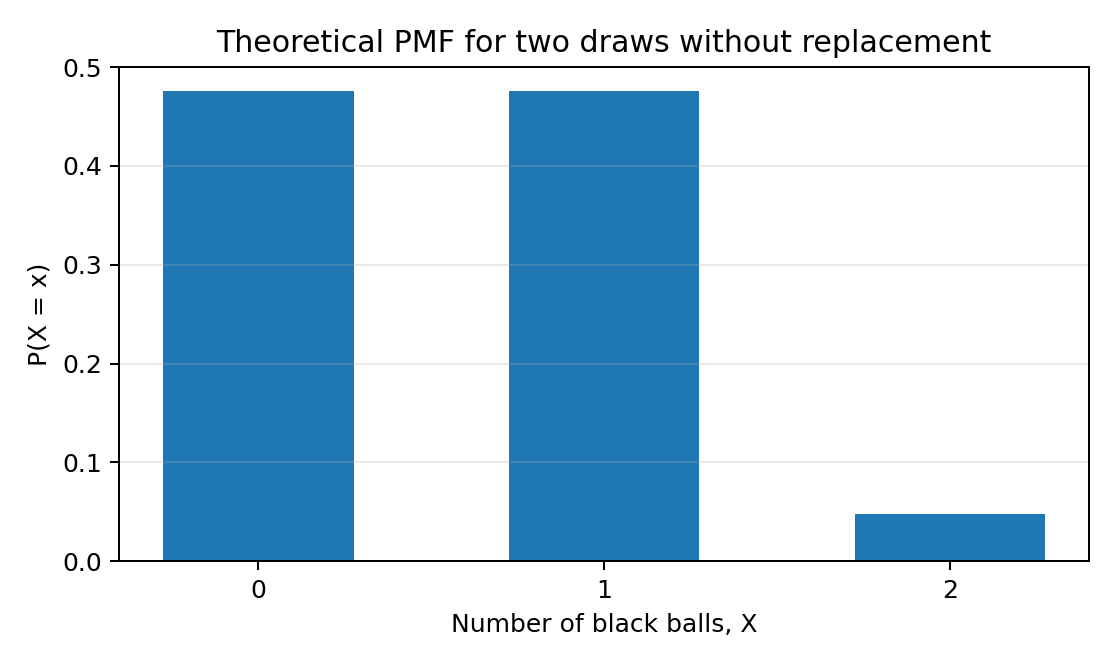
\includegraphics[width=0.90\linewidth]{figs/Q55_BlackBallsPMF.png}\end{figure}
\par\smallskip
\noindent\textbf{Code reference -- plotting and numerical verification}
\par\noindent\fbox{\parbox{\dimexpr\linewidth-2\fboxsep-2\fboxrule\relax}{\centering\texttt{codes/Q55.py}}}
\par\smallskip

\item[\textbf{1.2.56}] In 3 trials of a binomial distribution, the probability of exactly 2 successes is 9 times the probability of 3 successes. Find the success probability.
\solution Let the success probability be $p$ and $q=1-p$. The probability-generating polynomial is
\[
B(z)=(q+pz)^3=q^3+3pq^2z+3p^2qz^2+p^3z^3.
\]
The coefficient of $z^2$ is
\[
P(X=2)=\binom32p^2q=3p^2q,
\]
and the coefficient of $z^3$ is
\[
P(X=3)=p^3.
\]
Use $P(X=2)=9P(X=3)$:
\begin{align*}
3p^2q&=9p^3,\\
3p^2(1-p)&=9p^3.
\end{align*}
For the non-degenerate binomial case $p>0$, divide by $3p^2$: $1-p=3p$. Thus $4p=1$ and
\[
p=\frac14.
\]
The polynomial's coefficients directly identify the two probabilities; no separate $Z$-transform is needed beyond this generating-polynomial viewpoint.
\par\smallskip
\noindent\textbf{Code reference -- numerical verification}
\par\noindent\fbox{\parbox{\dimexpr\linewidth-2\fboxsep-2\fboxrule\relax}{\centering\texttt{codes/Q56.py}}}
\par\smallskip

\item[\textbf{1.2.57}] An urn contains 3 red and 5 black balls. A ball is drawn, its colour recorded and returned, and 2 more balls of that colour are added. Then two balls are drawn without replacement. Find the probability both are red.
\solution If the first ball is red, with probability $3/8$, the urn becomes 5 red and 5 black; the chance of two reds is $(5/10)(4/9)=2/9$. If the first ball is black, with probability $5/8$, the urn becomes 3 red and 7 black; the chance of two reds is $(3/10)(2/9)=1/15$. Thus
\[
P(\text{two red})=\frac38\frac29+\frac58\frac1{15}=\frac18.
\]
\par\smallskip
\noindent\textbf{Code reference -- numerical verification}
\par\noindent\fbox{\parbox{\dimexpr\linewidth-2\fboxsep-2\fboxrule\relax}{\centering\texttt{codes/Q57.py}}}
\par\smallskip

\item[\textbf{1.2.58}] A man speaks truth 3 out of 5 times. He throws a die and reports that it is 4. Find the probability that it actually is 4.
\solution Let $A$ be the event that the die shows 4, and $R$ the event that he reports 4. Assuming that when he lies each of the five wrong numbers is equally likely, $P(A)=1/6$, $P(R|A)=3/5$, and $P(R|A^c)=(2/5)(1/5)=2/25$. Hence
\[
P(A|R)=\frac{(1/6)(3/5)}{(1/6)(3/5)+(5/6)(2/25)}=\frac35.
\]
\end{enumerate}

\paragraph*{Linear programming}
\begin{enumerate}[label={},leftmargin=0pt,itemsep=9pt]
\item[\textbf{1.2.59}] Solve graphically: minimise $z=3x+5y$ subject to $x+2y\ge10$, $x+y\ge6$, $3x+y\ge8$, $x,y\ge0$.
\solution The lower-boundary vertices are $(0,8)$, $(1,5)$, $(2,4)$ and $(10,0)$. Their objective values are respectively $40$, $28$, $26$ and $30$. The smallest value is attained at $(2,4)$:
\[
x=2,\ y=4,\ z_{\min}=26.
\]
\begin{figure}[H]\centering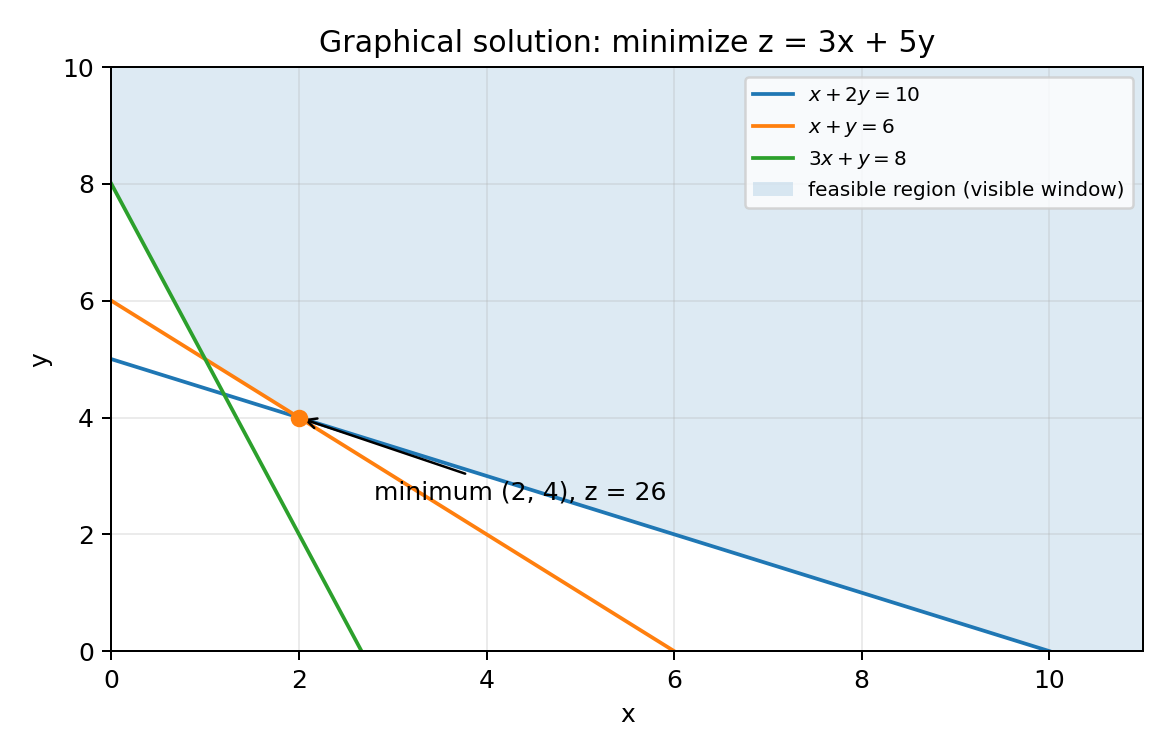
\includegraphics[width=0.92\linewidth]{figs/Q59_LPPMin.png}\end{figure}
\par\smallskip
\noindent\textbf{Code reference -- plotting and numerical verification}
\par\noindent\fbox{\parbox{\dimexpr\linewidth-2\fboxsep-2\fboxrule\relax}{\centering\texttt{codes/Q59.py}}}
\par\smallskip

\item[\textbf{1.2.60}] A dealer has Rs. 57,600 and space for at most 20 sewing machines. An electronic machine costs Rs. 3600 and earns Rs. 220 profit; a manual machine costs Rs. 2400 and earns Rs. 180 profit. How should he invest to maximise profit?
\solution Let $x$ and $y$ be electronic and manual machines. The constraints are $3x+2y\le48$, $x+y\le20$, $x,y\ge0$, and profit is $P=220x+180y$. At the intersection of the two active limits, $3x+2y=48$ and $x+y=20$, we get $(x,y)=(8,12)$ and $P=3920$. The axis vertices give profits Rs. 3520 and Rs. 3600. Therefore the best feasible integer plan is
\[
8\text{ electronic and }12\text{ manual machines; maximum profit Rs. }3920.
\]
\begin{figure}[H]\centering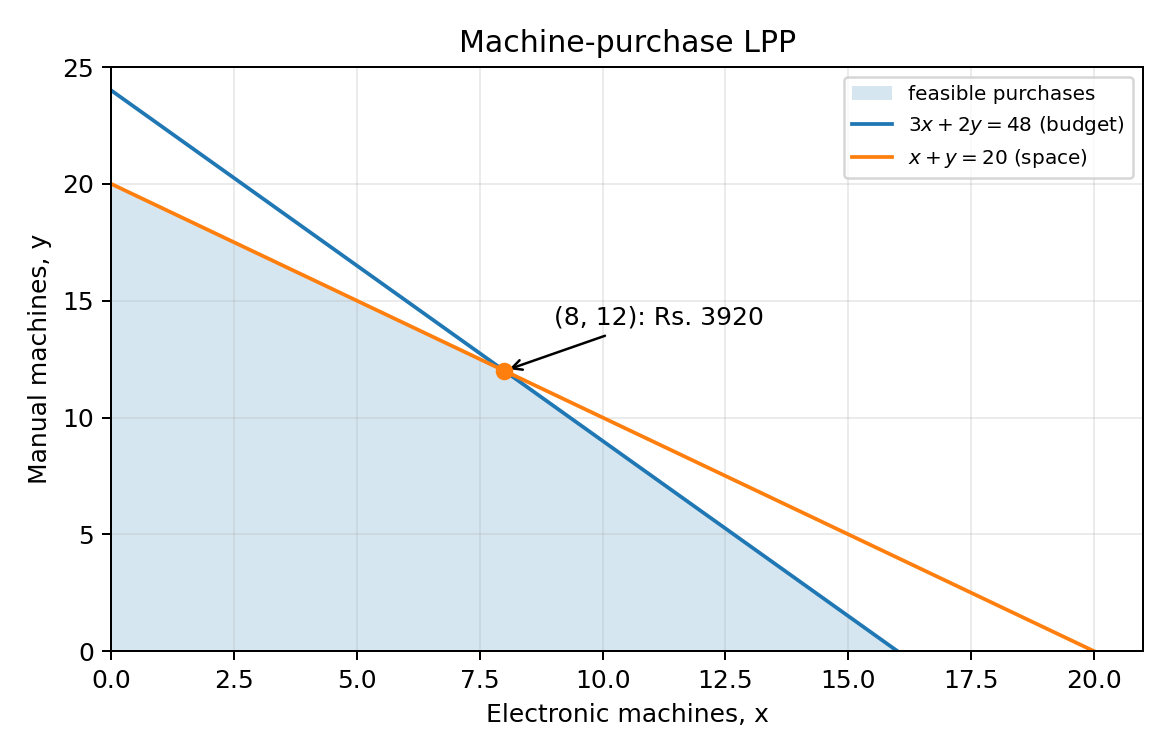
\includegraphics[width=0.92\linewidth]{figs/Q60_LPPProfit.png}\end{figure}
\par\smallskip
\noindent\textbf{Code reference -- plotting and numerical verification}
\par\noindent\fbox{\parbox{\dimexpr\linewidth-2\fboxsep-2\fboxrule\relax}{\centering\texttt{codes/Q60.py}}}
\par\smallskip
\end{enumerate}



\paragraph*{Coordinate geometry and optimisation}
\begin{enumerate}[label={},leftmargin=0pt,itemsep=9pt]
\item[\textbf{1.2.64}] A tangent to $x^2+y^2=4$ at a point in the first quadrant meets the positive axes at $A$ and $B$. Find the minimum of $OA+OB$.
\solution At the point $(2\cos\theta,2\sin\theta)$, the tangent is $x\cos\theta+y\sin\theta=2$. Thus $OA=2\sec\theta$ and $OB=2\csc\theta$. By symmetry (or differentiating), their sum is minimised when $\sin\theta=\cos\theta=1/\sqrt2$. Hence
\[
\min(OA+OB)=2(\sqrt2+\sqrt2)=4\sqrt2.
\]
\begin{figure}[H]\centering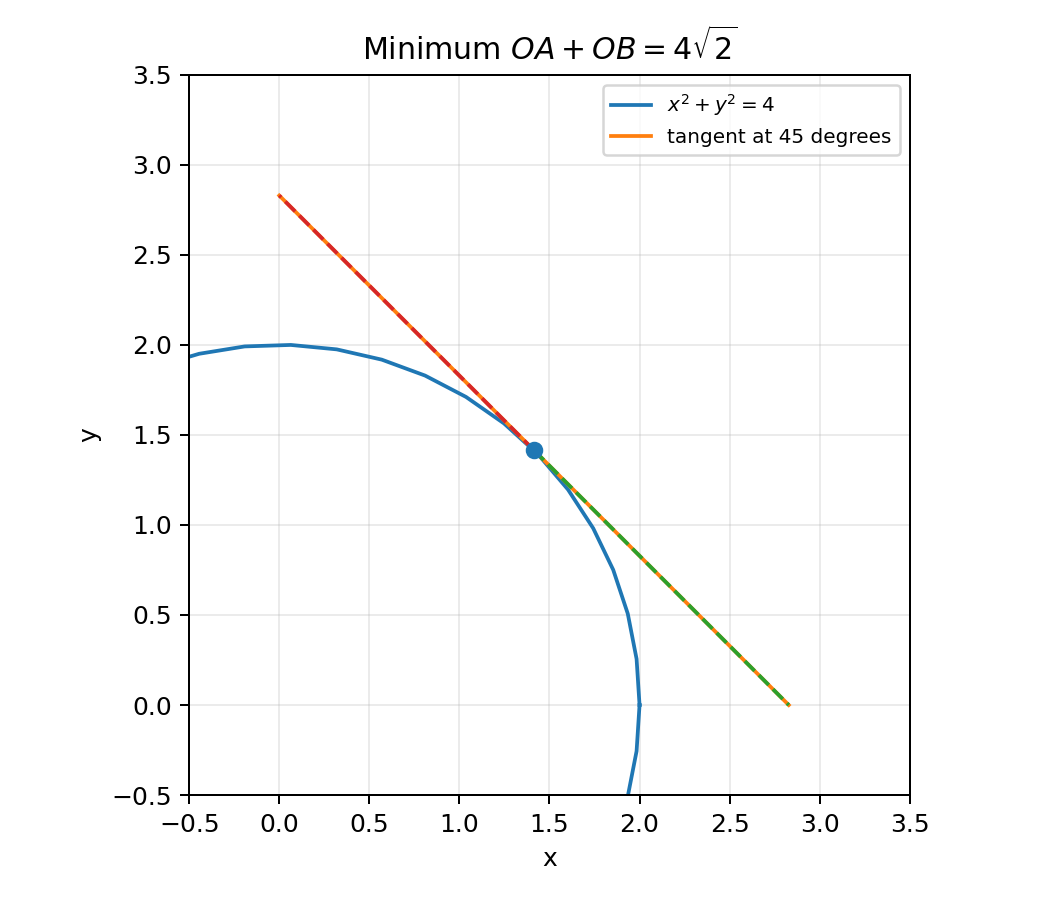
\includegraphics[width=0.92\linewidth]{figs/Q64_CircleTangent.png}\end{figure}
\par\smallskip
\noindent\textbf{Code reference -- plotting and numerical verification}
\par\noindent\fbox{\parbox{\dimexpr\linewidth-2\fboxsep-2\fboxrule\relax}{\centering\texttt{codes/Q64.py}}}
\par\smallskip

\item[\textbf{1.2.65}] Find the maximum area of an isosceles triangle inscribed in $\frac{x^2}{16}+\frac{y^2}{9}=1$ with its vertex at an end of the major axis.
\solution By symmetry, take the fixed vertex as $(4,0)$ and the other two vertices as $(u,v)$ and $(u,-v)$. From the ellipse, $v=3\sqrt{1-u^2/16}$. The area is
\[
A(u)=v(4-u)=3(4-u)\sqrt{1-u^2/16}.
\]
Differentiation gives $A'(u)=0$ when $u^2-2u-8=0$, i.e. $u=4$ or $u=-2$. The endpoint $u=4$ has zero area, so the maximum is at $u=-2$, where $v=3\sqrt3/2$. Thus
\[
A_{\max}=6\left(\frac{3\sqrt3}{2}\right)=9\sqrt3.
\]
\begin{figure}[H]\centering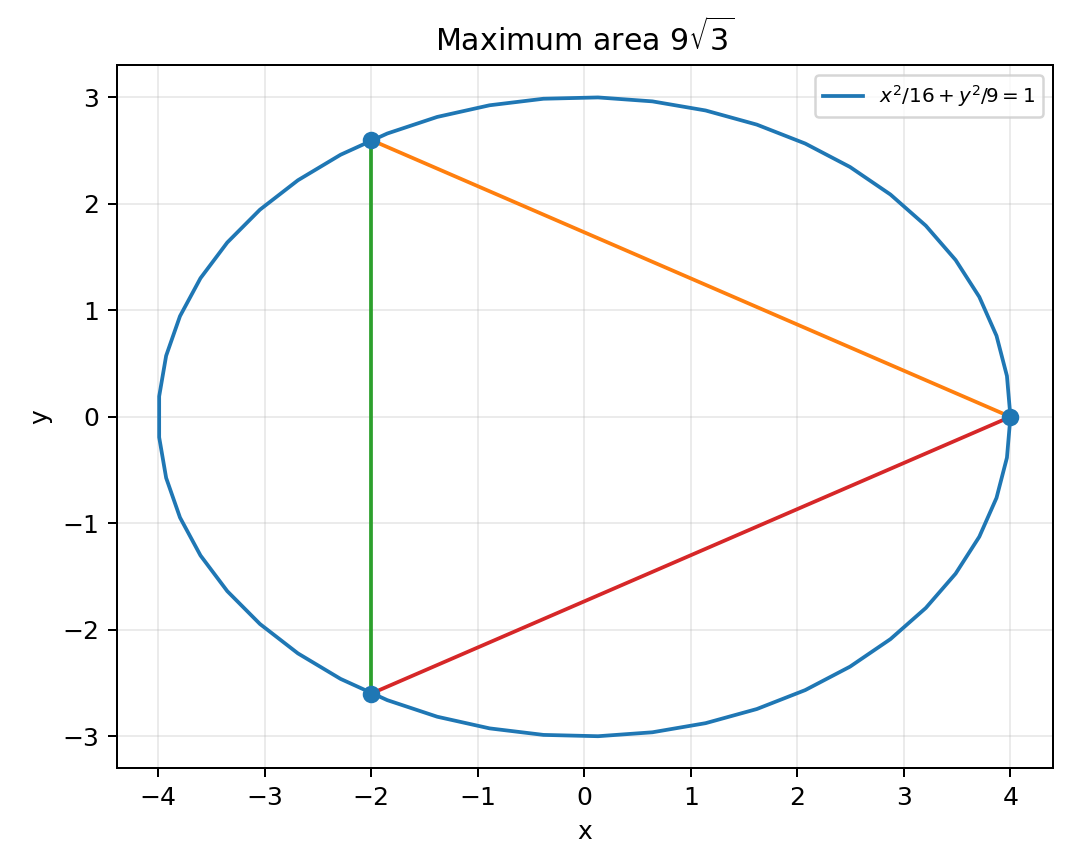
\includegraphics[width=0.92\linewidth]{figs/Q65_EllipseTriangle.png}\end{figure}
\par\smallskip
\noindent\textbf{Code reference -- plotting and numerical verification}
\par\noindent\fbox{\parbox{\dimexpr\linewidth-2\fboxsep-2\fboxrule\relax}{\centering\texttt{codes/Q65.py}}}
\par\smallskip
\end{enumerate}


\newpage
\end{document}
